\documentclass[11pt,a4paper]{article}
\usepackage{fontspec}
\IfFontExistsTF{Times New Roman}{\setmainfont{Times New Roman}}{\setmainfont{Liberation Serif}}
\IfFontExistsTF{Arial}{\setsansfont{Arial}}{\setsansfont{Liberation Sans}}
\IfFontExistsTF{Menlo}{\setmonofont[Scale=0.83]{Menlo}}{\setmonofont[Scale=0.83]{DejaVu Sans Mono}}
\usepackage[russian]{babel}
\usepackage[margin=25mm,headheight=14pt]{geometry}
\usepackage{amsmath,amssymb,amsthm,mathtools}
\usepackage{graphicx,booktabs,tabularx,array,longtable}
\usepackage{enumitem,xcolor,microtype}
\usepackage{fancyvrb,needspace}
\usepackage[unicode,colorlinks=true,linkcolor=blue!45!black,citecolor=blue!45!black,urlcolor=blue!45!black,bookmarksnumbered=true]{hyperref}
\usepackage{bookmark}
\hypersetup{pdftitle={Весовые системы хордовых диаграмм: мутации и продолжение на графы},pdfauthor={Димитрий Орехов}}
\graphicspath{{figures/}}
\setlength{\parindent}{1.25em}
\setlength{\parskip}{0.18em}
\setlength{\emergencystretch}{2em}
\setlist{nosep,topsep=4pt}
\allowdisplaybreaks
\numberwithin{equation}{section}
\newtheorem{theorem}{Теорема}[section]
\newtheorem{proposition}[theorem]{Утверждение}
\newtheorem{lemma}[theorem]{Лемма}
\theoremstyle{definition}
\newtheorem{definition}[theorem]{Определение}
\theoremstyle{remark}
\newtheorem*{remark}{Замечание}
\newcommand{\gl}{\mathfrak{gl}}
\newcommand{\sll}{\mathfrak{sl}}
\newcommand{\W}{W_{\gl}}
\newcommand{\F}{\mathbb F}
\newcommand{\Q}{\mathbb Q}
\newcommand{\Z}{\mathbb Z}
\newcommand{\Prim}{\operatorname{Prim}}
\newcommand{\corank}{\operatorname{corank}}
\newcommand{\rev}{\operatorname{rev}}
\newcommand{\Tr}{\operatorname{Tr}}
\newcommand{\rk}{\operatorname{rank}}
\newcommand{\repo}[2]{\href{https://github.com/TheMrX1/gl-weight-systems/blob/main/#1}{\texttt{\detokenize{#2}}}}
\newcommand{\file}[1]{\texttt{\detokenize{#1}}}
\title{Весовые системы хордовых диаграмм: мутации и продолжение на графы}
\author{Димитрий Орехов}
\date{20 ноября 2026 года}
\begin{document}
\maketitle

\section{Основные результаты}

Хордовая диаграмма порядка $n$ задаёт $n$ пар точек на окружности.
В её графе пересечений вершины соответствуют хордам, а рёбра соединяют
пересекающиеся хорды. Мутация перестраивает часть диаграммы
с сохранением этого графа. Универсальная $\gl$-весовая система
сопоставляет диаграмме многочлен от параметра $N$ и переменных Казимира
$C_1,C_2,\ldots$.

\begin{enumerate}[itemsep=.45em,topsep=.35em]
\item \textbf{Различающие веса в порядке 11.}
Построены две неизоморфные диаграммы-мутанты с 11 хордами. Их графы
пересечений совпадают, а универсальные $\gl$-веса различны.
Вычислены оба многочлена и их разность
(раздел~\ref{sec:mutants11}).

\item \textbf{Примитивные проекции той же пары.}
Примитивная проекция выделяет в алгебре диаграмм часть, остающуюся после
вычитания вкладов произведений диаграмм меньших порядков. У построенной
пары веса всех соответствующих собственных поддиаграмм совпадают,
поэтому проекция сохраняет разность весов
(раздел~\ref{sec:primitive}).

\item \textbf{Четыре разных веса в порядке 14.}
Построена диаграмма с 14 хордами, у которой исходная диаграмма и три
варианта мутации одной и той же доли дают четыре попарно различных
скалярных веса в неприводимом представлении $\gl_4$ с диаграммой Юнга
$(2,1)$. Следовательно, различны и четыре универсальных веса
(раздел~\ref{sec:mutants14}).

\item \textbf{Специализации по диаграммам Юнга.}
Неприводимое полиномиальное представление $\gl_N$ задаёт подстановку
собственных значений Казимиров в универсальный многочлен. Для пары
порядка 11 веса совпадают при каждой такой подстановке, соответствующей
прямоугольной диаграмме Юнга. Для крюков получена явная формула разности
и определены все параметры, при которых она равна нулю
(раздел~\ref{sec:young}).

\item \textbf{Диаграмма с полным графом пересечений.}
Для диаграммы из 11 попарно пересекающихся хорд вычислен полный
универсальный $\gl$-вес. Он содержит 587 мономов и включает зависимость
от $C_1$ (раздел~\ref{sec:complete}).

\item \textbf{Специализации графового сертификата порядка 9.}
Графовые $4T$-соотношения задают линейные тождества
между значениями функции на четвёрках графов. На опубликованной
комбинации таких соотношений~\cite{fkpu} хроматический многочлен
обнуляется. В представлении с квадратной диаграммой Юнга $(2,2)$
получены явные ненулевые веса комбинации и её примитивной проекции
для каждого $N\ge3$. Для полной хроматической подстановки найдены
17 ненулевых коэффициентов на той же комбинации
(раздел~\ref{sec:graph9}).

\item \textbf{Непродолжимость коэффициентов примитивного веса.}
В $\sll_2$-весе примитивной проекции выделим коэффициент
при $c^{\lfloor(n-1)/2\rfloor}$, где $c$ --- квадратичный Казимир для
формы Киллинга. В каждом из порядков 11, 12, 13 и 14 доказано, что
значения этого коэффициента на графах пересечений нельзя продолжить
на все графы того же порядка с сохранением графовых $4T$-соотношений
(раздел~\ref{sec:sl2}).
\end{enumerate}

\section{Постановка и обозначения}

\subsection{Хордовые диаграммы и графы пересечений}

Хордовая диаграмма порядка $n$ состоит из ориентированной окружности
и $n$ неупорядоченных пар различных точек на ней. Пары называются хордами.
В вычислениях диаграмма задаётся циклическим словом длины $2n$:
каждая метка встречается ровно дважды и соединяет соответствующие точки.
Например, слово $0101$ задаёт две пересекающиеся хорды, а $0011$ ---
две непересекающиеся. Геометрическое положение прямых отрезков внутри
круга не входит в определение; важен циклический порядок концов.

Граф пересечений $\Gamma(D)$ имеет по вершине на каждую хорду.
Две вершины смежны тогда и только тогда, когда концы соответствующих
хорд чередуются на окружности. Изоморфные графы пересечений не обязаны
задавать изоморфные хордовые диаграммы.

При сравнении диаграмм в этой работе допускаются циклический сдвиг,
перенумерация хорд и, дополнительно, обращение окружности. Таким образом,
проверенная ниже неизоморфность сохраняется и при более строгом соглашении,
требующем сохранять ориентацию. Каноническая форма слова получается
перенумерацией по первому появлению и выбором минимума среди всех сдвигов
слова и его обращения. Это конечная точная проверка изоморфности.

\subsection{Универсальная весовая система}

Используется следовая форма $B(X,Y)=\Tr(XY)$ на $\gl_N$.
Ей соответствует тензор
\[
 \Omega_{\gl}=\sum_{i,j=1}^N E_{ij}\otimes E_{ji}.
\]
Каждой хорде назначается копия этого тензора, а матричные единицы
перемножаются в порядке обхода окружности. Сумма по индексам принадлежит
центру универсальной обёртывающей алгебры. В универсальной записи её
значение является многочленом
\[
 \W(D)\in\Z[N,C_1,C_2,\ldots],\qquad C_0=N,
\]
где
\begin{equation}\label{eq:casimir}
 C_k=\sum_{i_1,\ldots,i_k=1}^N
 E_{i_1i_2}E_{i_2i_3}\cdots E_{i_ki_1},\qquad k\ge1.
\end{equation}
При фиксированном $N$ элементы центра имеют зависимости; универсальный
многочлен рассматривается до подстановки конкретного ранга и представления.
Для проверки формального неравенства допускаются любые целочисленные
значения независимых переменных, даже если они не реализуются центральным
характером представления.

В основе вычислителя лежит рекурсия для инварианта перестановок,
ограничение которого на инволюции без неподвижных точек даёт хордовой
$\gl$-вес \cite{yang}. Она реализует перестановку соседних генераторов
и поправки из соотношения
\begin{equation}\label{eq:commutator}
 [E_{ij},E_{kl}]=\delta_{jk}E_{il}-\delta_{il}E_{kj}.
\end{equation}
Получение новых примеров не требует изменения этого алгебраического
соотношения. Оптимизации касаются выбора представления промежуточных
результатов, повторного использования состояний и порядка вычислений.

\section{Численный и символьный вычислители}

\subsection{Почему можно вычислять значения, не выписывая многочлен}

Выберем простое $p$ и числа $a_0,a_1,\ldots\in\F_p$.
Отображение
\[
 \operatorname{ev}_{p,a}:\Z[N,C_1,C_2,\ldots]\longrightarrow\F_p,
 \qquad N\mapsto a_0,\quad C_i\mapsto a_i
\]
является гомоморфизмом колец. Поэтому оно коммутирует со всеми
сложениями, вычитаниями и умножениями исходной рекурсии. Вместо хранения
многочлена в каждом состоянии можно сразу хранить его значение в поле.
Итог совпадает с подстановкой в полностью вычисленный многочлен.

\begin{proposition}\label{prop:evaluation}
Если при одной и той же подстановке в одном поле значения двух
диаграмм различны, их универсальные многочлены различны.
\end{proposition}
\begin{proof}
Равные многочлены имеют равные образы при любом гомоморфизме колец.
Применяем контрапозицию этого утверждения.
\end{proof}

Ненулевая разность является строгим свидетельством. Совпадение значений
в нескольких точках не является доказательством равенства многочленов.
В работе равенства, на которых основаны дальнейшие выводы, проверяются
сравнением всех коэффициентов либо отдельным алгебраическим тождеством.

По умолчанию численный вычислитель использует три поля с модулями
\[
 1000000007,\qquad1000000009,\qquad998244353.
\]
Подстановки детерминированы: последовательность SplitMix64 с фиксированным
начальным состоянием задаёт значения Казимиров по правилу
$C_i=1+(r_i\bmod(p-1))$. Точное начальное состояние, включая преобразования
параметра запуска, фиксировано в исходниках; оно не зависит от машины
или числа потоков. Вычислитель выводит сами модули и все значения
переменных, поэтому результат воспроизводим без догадок о генераторе.
Режим $C_1=0$ является только специализацией универсального многочлена;
его нельзя отождествлять с полной $\sll_2$-весовой системой.

\subsection{Как устроено символьное вычисление}

Символьный вариант сначала строит ациклический граф операций, а затем
раскрывает нужные узлы в многочлены. Одинаковые рекурсивные состояния
используют общий результат; промежуточное выражение освобождается после
последнего обращения к нему. Степени мономов кодируются компактно.
В варианте для больших вычислений одинаковые многочлены хранятся в одном
экземпляре, а ранги мономов и коэффициенты записываются обратимым
целочисленным кодированием. Совпадение хешей само по себе не считается
равенством: сравнивается полная каноническая кодировка.

Численный вариант заменяет операции над списками мономов несколькими
операциями над числами. Символьный вариант сокращает повторные вычисления
и время жизни промежуточных выражений. Ускорение зависит от диаграммы:
сам порядок $n$ не определяет число рекурсивных состояний. Обращение
обхода окружности сохраняет Lie-вес хордовой диаграммы, но может менять
объём промежуточной рекурсии; поэтому оно также используется при выборе
удобного входного слова.

Арифметика универсального символьного ядра точна в установленном диапазоне:
выход за поддерживаемые разрядности вызывает ошибку, а не молчаливое
переполнение. В вычислителях $\sll_2$, центральных характеров и рациональных
сертификатов используются целые числа произвольной точности. Нельзя
выдавать ограничения одного из этих вычислителей за ограничения остальных.

Независимые проверки включали прямые матричные свёртки, реализацию
соотношения \eqref{eq:commutator}, сравнение полных многочленов на малых
и средних порядках, проверку подстановок уже полученных выражений и
запуски с контролем выхода за границы памяти и неопределённого поведения.
Это проверки реализации известной рекурсии, а не новая теорема о ней.


\section{Мутанты порядка 11 с различными универсальными весами}
\label{sec:mutants11}

\subsection{Доля и операции мутации}

Пусть слово диаграммы разбито на четыре последовательных блока
$D=ABCE$. Концы хорд выбранной доли лежат в $A,C$, а концы остальных
хорд --- в $B,E$. Множества меток двух групп не пересекаются.
Обозначим
\begin{equation}\label{eq:mutations}
 \begin{split}
 R(D)&=\rev(A)\,B\,\rev(C)\,E,\\
 S(D)&=CBAE,\\
 RS(D)&=\rev(C)\,B\,\rev(A)\,E.
 \end{split}
\end{equation}
Здесь $\rev$ обращает порядок концов внутри блока. Операции $R,S$ ---
коммутирующие инволюции. Они сохраняют граф пересечений; связь мутаций
и графов пересечений рассматривается в \cite{chmutovlando}.

Для найденной пары блоки имеют вид
\[
 \begin{array}{ll}
 A=(0\ 1\ 2\ 0\ 3\ 1\ 2),&B=(4\ 5\ 6\ 7\ 8\ 5\ 9\ 4\ 8\ 10),\\
 C=(3),&E=(7\ 9\ 10\ 6).
 \end{array}
\]
Доля $A,C$ содержит четыре хорды, дополнение --- семь. Получены слова
\begin{equation}\label{eq:words11}
\begin{aligned}
D={}&(0\ 1\ 2\ 0\ 3\ 1\ 2\ 4\ 5\ 6\ 7\ 8\ 5\ 9\ 4\ 8\ 10\ 3\ 7\ 9\ 10\ 6),\\
D'={}&(3\ 4\ 5\ 6\ 7\ 8\ 5\ 9\ 4\ 8\ 10\ 0\ 1\ 2\ 0\ 3\ 1\ 2\ 7\ 9\ 10\ 6).
\end{aligned}
\end{equation}
Итак, $D'=S(D)$. Неизоморфность проверяется канонизацией циклических
слов; размеченные графы пересечений совпадают буквально.

\begin{figure}[htbp]
\centering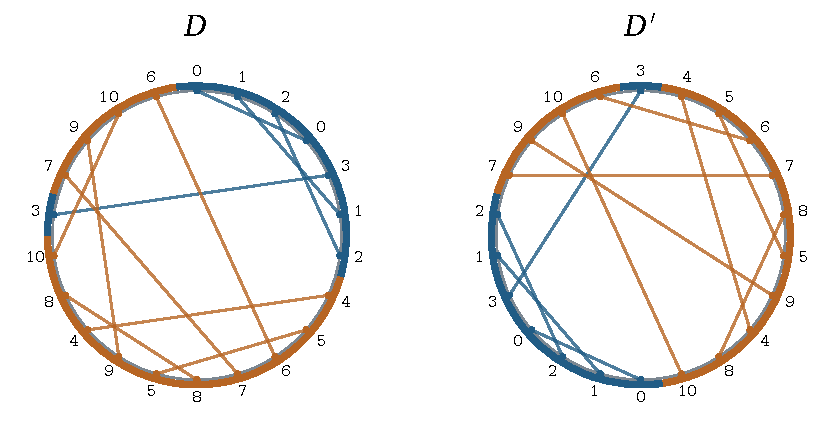
\includegraphics[width=\linewidth]{mutants11.pdf}
\caption{Пара \eqref{eq:words11}. Синим выделена четырёххордовая доля,
оранжевым --- дополнение. Слова читаются от верхней точки по часовой
стрелке. При мутации меняются местами две синие дуги.}
\label{fig:pair}
\end{figure}

\subsection{Поиск через операторы долей}

Поиск можно организовать так, чтобы дорогая часть вычислялась для каждой
доли отдельно. Для выбранного представления $V$ положим
\[
 T_{A,C}=\sum\rho(A)\otimes\rho(C)\in\operatorname{End}(V\otimes V),
\]
где сумма идёт по назначениям индексов хордам доли. Аналогично строится
$T_{B,E}$. Тогда тождество
$\Tr(P(L\otimes M))=\Tr(LM)$ даёт
\[
 w_V(ABCE)=\frac1{\dim V}\Tr_{V\otimes V}
 \bigl(P\,T_{A,C}T_{B,E}\bigr).
\]
Это точная формула сшивания. Операторы можно переиспользовать при
переборе различных партнёров, вместо повторного вычисления полного
универсального веса каждой пары. В разложении $V\otimes V$ инвариантные
операторы действуют на пространствах кратностей; именно там сохраняется
информация, которую может менять мутация. Для $V_{(2,1)}$ размерности 20
в разложении имеется 64-мерная компонента кратности два.

Реализован разреженный расчёт блоков долей с выбором порядка обработки
концов, уменьшающего число одновременно открытых хорд. Предварительный
детектор использует конечномерную специализацию; найденные кандидаты
после этого проверяются универсальной рекурсией и полными многочленами.
Так получена пара с разбиением $4+7$. Полнота перебора всех мутантов
порядка 11 для предъявления этого примера не требуется и не заявляется.

\subsection{Точный результат}

Полные многочлены $\W(D)$ и $\W(D')$ содержат по 521 ненулевому моному.
Их разность $\Delta=\W(D)-\W(D')$ содержит 27 мономов и зависит только
от $N,C_1,\ldots,C_6$. В формальной подстановке
\begin{equation}\label{eq:formal}
 N=1,\qquad C_2=1,\qquad C_i=0\quad(i\ge1,\ i\ne2)
\end{equation}
получаем
\[
 \W(D)=11342,\qquad \W(D')=11322,\qquad\Delta=20.
\]
Это непосредственно доказывает неравенство универсальных многочленов.
Подстановка \eqref{eq:formal} не является одномерным представлением
$\gl_1$ и не используется в таком качестве.

Есть и свидетельство в настоящем представлении. Для неприводимого
$\gl_4$-модуля с диаграммой Юнга $(2,1)$ и размерностью 20 имеем
\[
 (N,c_1,c_2,c_3,c_4)=(4,3,12,51,228).
\]
Специализация универсальной разности даёт $-423360$. Она также проверена
прямой матричной свёрткой определения весовой системы. Таким образом,
различие не является особенностью формальной подстановки.

Готовые полные многочлены находятся в
\repo{results/mutants11/D_ordinary.json}{results/mutants11/}.
JSON хранит коэффициент десятичной строкой и массив степеней:
нулевая позиция соответствует $N$, позиция $k$ --- $C_k$.
Символьный расчёт исходной пары занял в одном из зафиксированных запусков
177{,}49 с при максимальном RSS около 7{,}96 ГБ. Это измерение данной
пары, а не оценка любого входа порядка 11.

\Needspace{12\baselineskip}
\section{Проекция на примитивные элементы}
\label{sec:primitive}

\subsection{Алгебра Хопфа и формула проекции}

Пусть $\mathcal A$ --- градуированная алгебра хордовых диаграмм по модулю
хордовых 4T-соотношений. Произведение задаётся склейкой окружностей,
а копроизведение диаграммы с множеством хорд $V$ равно
\[
 \delta(D)=\sum_{U\subseteq V}D_U\otimes D_{V\setminus U}.
\]
Примитивный элемент $x$ удовлетворяет
$\delta(x)=1\otimes x+x\otimes1$.
В связной коммутативной кокоммутативной алгебре Хопфа над $\Q$
каноническая проекция на примитивную часть задаётся свёрточным
логарифмом $\pi=\log_*\operatorname{Id}$. Для непустой диаграммы
\begin{equation}\label{eq:primitive}
 \pi(D)=\sum_{\rho\vdash V}
 (-1)^{|\rho|-1}(|\rho|-1)!\prod_{U\in\rho}D_U.
\end{equation}
Сумма идёт по неупорядоченным разбиениям на непустые блоки.
Коэффициент получается из ряда логарифма: упорядоченные $k$ блоков
дают $k!$ одинаковых произведений, а множитель ряда равен
$(-1)^{k-1}/k$. Поэтому остаётся $(-1)^{k-1}(k-1)!$.

Проекция $\pi(D)$ обычно является линейной комбинацией диаграмм,
а не отдельной диаграммой. Она не получается удалением некоторых
внешне <<непримитивных>> мономов из уже выписанного gl-многочлена.

\subsection{Моменты и кумулянты}

Положим $m(U)=\W(D_U)$, $m(\varnothing)=1$ и
$\kappa(U)=\W(\pi(D_U))$. Из мультипликативности веса следует
\begin{equation}\label{eq:cumulant}
 \kappa(V)=\sum_{\rho\vdash V}(-1)^{|\rho|-1}(|\rho|-1)!
 \prod_{U\in\rho}m(U).
\end{equation}
Для практического расчёта фиксируем $a\in V$ и выделяем блок,
содержащий $a$. Получаем якорную рекурсию
\begin{equation}\label{eq:anchor}
 \kappa(V)=m(V)-\sum_{\substack{U\subsetneq V\\a\in U}}
 \kappa(U)m(V\setminus U).
\end{equation}
Это обращение обычной связи моментов и кумулянтов. Оно справедливо в любом
коммутативном кольце, поэтому одинаково применимо к многочленам и их
значениям в полях.

Для всех подмножеств требуется $O(3^n)$ операций в кольце и $O(2^n)$
значений. Число слагаемых в суммах \eqref{eq:anchor} равно
\[
 \frac{3^n-2^{n+1}+1}{2};\qquad n=11:\quad86526.
\]
В эту оценку не входит получение самих моментов $m(U)$; для символьных
операций дополнительно важен размер многочленов.

\subsection{Результат для найденной пары}

Для каждого из 2046 непустых собственных подмножеств множества меток
проверено точное равенство
\[
 \W(D_U)=\W(D'_U).
\]
Если разбиение в \eqref{eq:cumulant} имеет больше одного блока,
каждый его блок является собственным подмножеством. Все соответствующие
произведения совпадают. Следовательно,
\begin{equation}\label{eq:primitive-difference}
 \W(\pi(D))-\W(\pi(D'))=\W(D)-\W(D')=\Delta\ne0.
\end{equation}
Это специальное свойство данной пары. Равенство $\W(\pi(D))=\W(D)$
для произвольной диаграммы не утверждается и, вообще говоря, неверно.

Оба примитивных многочлена содержат по 138 мономов. Общая поправка
$\W(D)-\W(\pi(D))$ содержит 443 монома. Подстановка \eqref{eq:formal}
даёт $-4888$ и $-4908$; разность по-прежнему равна 20.
В представлении $(2,1)$ алгебры $\gl_4$ примитивные значения равны
$-4807971744$ и $-4807548384$, разность равна $-423360$.

Формула проекции дополнительно проверена независимым перебором всех
678570 разбиений 11 хорд. Проверены также примитивность копроизведения
в малых порядках и обнуление проекции произведений положительных степеней.
Полные примитивные многочлены и поправка опубликованы рядом с обычными.

\section{Четыре мутации одной доли}
\label{sec:mutants14}

Для исходной четырёххордовой доли обозначим $D''=R(D)$ и $D'''=RS(D)$.
Все четыре диаграммы попарно неизоморфны, но их универсальные веса
образуют две группы:
\begin{equation}\label{eq:four11}
 \W(D)=\W(D''),\qquad\W(D')=\W(D'''),\qquad\W(D)\ne\W(D').
\end{equation}
Та же таблица верна после проекции на примитивные. Эти равенства
проверены по всем коэффициентам, а не только в конечных полях.

Для дополнительной семихордовой доли операции обращают или переставляют
блоки $B,E$. Обращение этих двух дуг даёт
$M=A\rev(B)C\rev(E)$. Глобальное обращение $M$ с циклическим сдвигом
совпадает с $D'''$. Перестановка $B,E$ циклически совпадает с $D'$.
Поэтому для этой доли таблица весов имеет вид
\[
 \begin{array}{c|rrrr}
 \text{операция}&1&R&S&RS\\\hline
 \text{вес}&p&q&q&p
 \end{array}\qquad(p\ne q).
\]
Значит, обе базисные операции $R$ и $S$ могут менять вес на одной и той же
доле. Гипотеза об универсальной инвариантности одной из них неверна.

Более сильный пример получен в порядке 14. Выберем блоки
\[
\begin{array}{ll}
 A=(0\ 1\ 2\ 3\ 4\ 1\ 5\ 0\ 4\ 6),&
 B=(13\ 11\ 12\ 9\ 7\ 8\ 11\ 7\ 10\ 8),\\
 C=(3\ 5\ 6\ 2),&E=(10\ 13\ 12\ 9).
\end{array}
\]
Доля и дополнение содержат по семь хорд. В том же настоящем
20-мерном представлении $V_{(2,1)}$ алгебры $\gl_4$ имеем
\begin{center}
\begin{tabular}{cr}
\toprule
Диаграмма&Скалярный вес $w_V$\\\midrule
$X=ABCE$&1111487173017\\
$R(X)$&1111489713177\\
$S(X)$&1111487850393\\
$RS(X)$&1111485310233\\\bottomrule
\end{tabular}
\end{center}
Все четыре значения различны. Следовательно, даже выбор сохраняющей
мутации из всех трёх нетривиальных операций не всегда возможен.
Минимальность порядка 14 этим примером не устанавливается.

Здесь $w_V(D)$ --- скаляр действия центрального элемента на
неприводимом модуле, то есть
\[
 \rho(\W(D))=w_V(D)\operatorname{Id}_V,
 \qquad w_V(D)=\frac{\Tr\rho(\W(D))}{\dim V}.
\]
Это специализация универсальной gl-весовой системы, поэтому различие
скаляров строго доказывает различие универсальных весов.

\begin{figure}[p]
\centering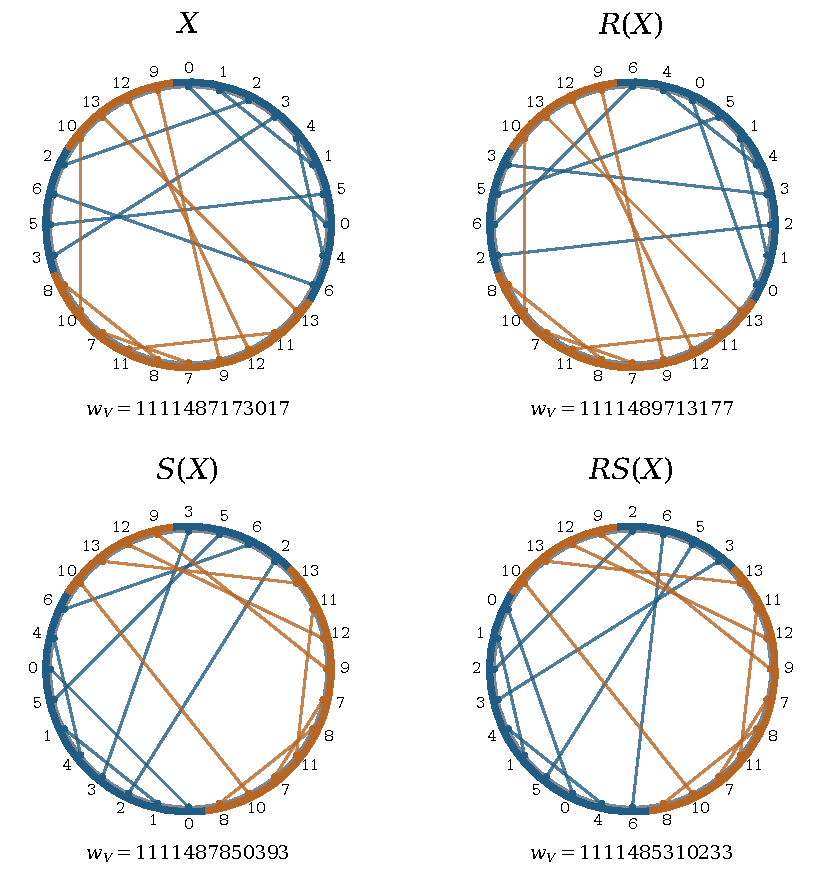
\includegraphics[width=.92\linewidth]{mutants14.pdf}
\caption{Мутационная четвёрка порядка 14. Все диаграммы имеют один и тот же
размеченный граф пересечений. Цвет выделяет выбранную долю и дополнение.
Подписи $w_V$ относятся к модулю $V_{(2,1)}$ алгебры $\gl_4$.}
\label{fig:four14}
\end{figure}

Числа получены полной тензорной свёрткой, без универсальной gl-рекурсии.
Модуль реализован как
\[
 V=\ker\bigl(\operatorname{Sym}^2\mathbb C^4\otimes\mathbb C^4
 \longrightarrow\operatorname{Sym}^3\mathbb C^4\bigr).
\]
Для его целочисленных матриц проверены все 256 соотношений
\eqref{eq:commutator}. На $V\otimes V$ проверен полный ранг 400
базиса тензорных компонент; повторяющийся 64-мерный тип сохраняется
с обеими копиями. Значения восстановлены по пяти простым модулям.
Произведение модулей превосходит удвоенную доказанную оценку абсолютного
значения, поэтому китайская теорема об остатках определяет единственное
целое, а не только наиболее правдоподобный ответ.

\section{\texorpdfstring{Представления $\gl_N$ и диаграммы Юнга}{Представления gl(N) и диаграммы Юнга}}
\label{sec:young}

\subsection{Переход от формы к центральному характеру}

Неприводимые полиномиальные представления $\gl_N$ нумеруются
разбиениями $\lambda=(\lambda_1\ge\cdots\ge\lambda_N\ge0)$.
Диаграмма Юнга имеет $\lambda_i$ клеток в строке $i$; нулевые строки
обычно не рисуют. Число хорд $n$, ранг $N$ и число клеток
$|\lambda|$ --- три разных параметра.

Положим $l_i=\lambda_i+N-i$. В нормировке \eqref{eq:casimir}
центральные характеры $c_m$ определяются производящей формулой
Переломова--Попова, согласованной с проекцией Хариш--Чандры
\cite{yang}:
\begin{equation}\label{eq:pp}
 1-Nz-\sum_{m\ge1}c_m z^{m+1}
 =\prod_{i=1}^{N}\frac{1-(l_i+1)z}{1-l_i z}.
\end{equation}
Для нужной специализации достаточно вычислить коэффициенты этого
формального ряда и подставить их в универсальный многочлен.
Матрицы всего представления могут при этом иметь огромную размерность;
строить их для каждого вычисления не требуется.

\begin{figure}[htbp]
\centering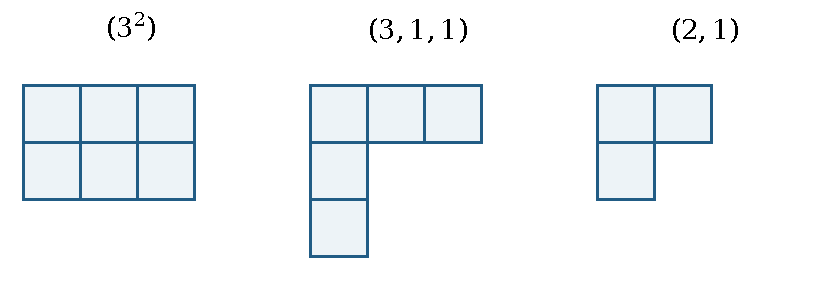
\includegraphics[width=.82\linewidth]{young.pdf}
\caption{Прямоугольник $(3^2)$ и крюки $(3,1,1)$, $(2,1)$.
У крюка $\lambda=(a,1^{b-1})$ длина верхней строки равна $a$,
высота первого столбца --- $b$.}
\end{figure}

\subsection{Все прямоугольные специализации найденной пары}

Для $\lambda=(a^b)$, где $a\ge1$ и $1\le b\le N$, произведение
\eqref{eq:pp} телескопируется:
\[
 \frac{(1-(N+a)z)(1-(N-b)z)}{1-(N+a-b)z}
 =1-Nz-\frac{abz^2}{1-(N+a-b)z}.
\]
Следовательно,
\begin{equation}\label{eq:rectangle-casimirs}
 c_m((a^b);N)=ab(N+a-b)^{m-1}.
\end{equation}

Для универсальной разности найденной пары проверено формальное тождество
\begin{equation}\label{eq:geometric}
 \left.\Delta\right|_{C_m=xy^{m-1}}=0\quad\text{в }\Z[N,x,y].
\end{equation}
Проверка состоит в группировке 27 мономов по степеням
$(N,x,y)$: получаются девять групп, сумма коэффициентов каждой равна нулю.
Подстановка $x=ab$, $y=N+a-b$ и \eqref{eq:primitive-difference} дают
\begin{proposition}
Для найденной пары $D,D'$ и каждого допустимого прямоугольника
$(a^b)$ совпадают как обычные веса, так и веса примитивных проекций.
Число клеток прямоугольника не ограничивается.
\end{proposition}
По \eqref{eq:four11} это верно и для всей исходной четвёрки.
Доказательство использует тождество \eqref{eq:geometric}, а не
экстраполяцию сетки размеров. Оно относится к фиксированной паре
и само по себе не доказывает утверждения для всех мутантов.

\subsection{Общая формула для крюков}

Для $\lambda=(a,1^{b-1})$ положим $s=a+b-1$.
Сокращение соседних множителей в \eqref{eq:pp} даёт
\[
 1-Nz-\sum_{m\ge1}c_m z^{m+1}
 =\frac{(1-(N+a)z)(1-Nz)(1-(N-b)z)}
 {(1-(N+a-1)z)(1-(N-b+1)z)}.
\]
Если $a+b>2$, то
\begin{equation}\label{eq:hook-casimirs}
 c_m=\frac{a+b-1}{a+b-2}
 \left((a-1)(N+a-1)^{m-1}+(b-1)(N-b+1)^{m-1}\right).
\end{equation}
При $a=b=1$ отдельно имеем $c_m=N^{m-1}$.

Ключевое конечное алгебраическое тождество имеет вид
\begin{equation}\label{eq:twoatom}
\begin{split}
 \left.\Delta\right|_{C_m=AX^{m-1}+BY^{m-1}}
 ={}&20AB(X-Y)^2(AY+BX-NXY)\\
 &\cdot\bigl(3(A+B)+N^2-N(X+Y)\bigr)^2.
\end{split}
\end{equation}
Оно проверено по всем 69 ненулевым коэффициентам раскрытых частей
независимой разреженной целочисленной арифметикой. Короткую проверку
можно выполнить без системы компьютерной алгебры.

Подставим
\[
 X=N+a-1,\quad Y=N-b+1,\quad
 A=\frac{s(a-1)}{a+b-2},\quad B=\frac{s(b-1)}{a+b-2}.
\]
Тогда $AB(X-Y)^2=s^2(a-1)(b-1)$,
$AY+BX=sN$,
$AY+BX-NXY=-N(N-b)(N+a)$.
Последний квадрат в \eqref{eq:twoatom} равен
$\bigl(N(N+a-b)-3s\bigr)^2$. Получаем:

\begin{theorem}\label{thm:hook}
Для фиксированной пары \eqref{eq:words11} и всех целых
$N\ge1$, $a\ge1$, $1\le b\le N$ разность скалярных весов равна
\begin{equation}\label{eq:hook-delta}
\begin{split}
 \Delta_{N,a,b}={}&-20N(N-b)(N+a)(a-1)(b-1)(a+b-1)^2\\
 &\cdot\bigl(N(N+a-b)-3(a+b-1)\bigr)^2.
\end{split}
\end{equation}
Та же формула верна для разности весов примитивных проекций.
\end{theorem}

Формула классифицирует все крюковые специализации этой пары.
При $N\le3$ каждая допустимая специализация даёт нуль.
При $N\ge4$ нулевые случаи в точности таковы:
\[
 a=1,\qquad b=1,\qquad b=N,\qquad (a,b)=(2,N-1).
\]
В остальных случаях разность строго отрицательна. Для доказательства
последнего утверждения достаточно перегруппировать множитель:
\[
 N(N+a-b)-3(a+b-1)
 =(N-3)(a-2)+(N+3)(N-b-1).
\]
Во внутренней области $a\ge2$, $2\le b\le N-1$ оба слагаемых
неотрицательны, а при $N\ge4$ обращаются в нуль одновременно только
при $a=2,b=N-1$.

Для равных плеч $a=b=k$ имеем
\[
 \Delta_{N,k,k}=-20N(N^2-k^2)(k-1)^2(2k-1)^2(N^2-6k+3)^2.
\]
При $k\ge3$ разность ненулевая для каждого $N\ge k+1$.
В частности, $\Delta_{4,2,2}=-423360$ и
$\Delta_{4,3,3}=-56000$. Это бесконечные семейства специализаций,
различающих одну и ту же пару порядка 11.

Есть дополнительный результат для малых рангов: универсальная
разность этой пары равна нулю в $Z(U(\gl_N))$ при $N=1,2,3$.
Для проверки подставляются независимые старшие веса в
\eqref{eq:pp}; полученный образ $\Delta$ тождественно нулевой.
Инъективность проекции Хариш--Чандры на центре даёт равенство
самих центральных элементов. Следовательно, минимальный ранг,
различающий именно эту пару, равен 4. Это не утверждение о любых
парах мутантов ранга 3.

\section{\texorpdfstring{Полный многочлен диаграммы $K_{11}$}{Полный многочлен диаграммы K11}}
\label{sec:complete}

Обозначим через $K_n$ диаграмму со словом
$0\,1\,\ldots\,(n-1)\,0\,1\,\ldots\,(n-1)$.
Её граф пересечений полный; каждая $k$-хордовая поддиаграмма
изоморфна $K_k$. Это позволяет использовать центральное разложение
$\gl_N=\sll_N\oplus\mathbb C I$ без перечисления различных типов
поддиаграмм.

Положим $z=C_1^2/N$ и
\begin{equation}\label{eq:shifted}
 D_j=\sum_{l=0}^{j}\binom jl
 \left(-\frac{C_1}{N}\right)^{j-l}C_l,\qquad C_0=N.
\end{equation}
Это циклические Казимиры матрицы $E-(C_1/N)I$, причём $D_1=0$.
Если $T_k=\W(K_k)|_{C_1=0}$ и $T_0=1$, то
\begin{equation}\label{eq:complete}
 \W(K_n)=\sum_{k=0}^n\binom nk z^{n-k}
 T_k(N,D_2,D_3,\ldots).
\end{equation}
Действительно, тензор следовой формы разлагается как
$\Omega_{\gl}=\Omega_{\sll}+I\otimes I/N$.
Выбор центрального слагаемого на $n-k$ хордах даёт $z^{n-k}$;
оставшаяся диаграмма --- $K_k$. Число таких выборов равно $\binom nk$.
Формула \eqref{eq:shifted} следует из обычной биномиальной формулы,
поскольку центральная скалярная матрица коммутирует со всеми элементами.

Расчёт восстановления выполняется в кольце многочленов Лорана по $N$;
все отрицательные степени в итоге сокращаются, что проверяется явно.
Получен полный $\W(K_{11})$ с независимым $C_1$: он содержит
587 мономов. Вспомогательный $T_{11}$ содержит 195 мономов.
Это разные выражения; специализация $C_1=0$ не подменяет полный ответ.

Для независимой проверки используется тождество
\[
 \Tr_{V\otimes V}(P\Omega^n)=\Tr_V\rho(\W(K_n)),
 \qquad P(u\otimes v)=v\otimes u.
\]
Оно следует раскрытием произведения и не использует рекурсию перестановок.
В 12 точных матричных специализациях итог совпал с полным многочленом.
Также коэффициент за коэффициентом проверены тождества
\[
 \left.\W(K_{11})\right|_{C_k=N^{k-1}}=N,\qquad
 \left.\W(K_{11})\right|_{C_k=Nt^k}=(Nt^2)^{11}.
\]

Разворачивание сохранённого графа бесследовой специализации в одном
измеренном запуске заняло 629{,}50 с при максимальном RSS около
12 ГиБ. Это время отдельного этапа. Сжатые промежуточные данные занимали
около 4{,}68 ГБ; хранение тех же пар по 16 байт потребовало бы около
28{,}4 ГБ только на слагаемые. Итог и вспомогательные $T_1,\ldots,T_{11}$
позволяют повторить точное восстановление без нового большого расчёта.

\section{Графовые 4T и хроматическая подстановка}
\label{sec:graph9}

\subsection{Две разные постановки}

Вес может зависеть только от графа пересечений, но не продолжаться
на все простые графы с сохранением графовых 4T. Это разные условия.
В первом случае значения согласованы на графах, реализуемых хордовыми
диаграммами; во втором требуется выполнить дополнительные отношения,
в которых встречаются и не реализуемые таким образом графы.

Для разных вершин $a,b$ обозначим через $G'_{ab}$ переключение ребра $ab$.
Граф $\widetilde G_{ab}$ получается переключением рёбер от $a$ ко всем
соседям $b$, кроме самих $a,b$; ребро $ab$ сохраняется.
Функция $f$ является графовым 4-инвариантом, если
\begin{equation}\label{eq:graph4t}
 f(G)-f(G'_{ab})-f(\widetilde G_{ab})+f(\widetilde G'_{ab})=0.
\end{equation}
Пусть $\mathcal H$ --- алгебра Хопфа графов по модулю этих отношений.
Отображение $\Gamma:\mathcal A\to\mathcal H$ согласуется с произведением,
копроизведением и примитивной проекцией.

В \cite{fkpu} построена комбинация графовых 4T на девяти вершинах,
которая после сокращений состоит из 5006 графов пересечений.
Выберем указанные авторами хордовые реализации и обозначим их
линейную комбинацию через $L_9$. Тогда
\[
 \Gamma(L_9)=0\quad\text{в }\mathcal H,
\]
но её $\sll_2$-вес с формой Киллинга равен
\begin{equation}\label{eq:r9}
 R(c)=c\left(c+\frac3{32}\right)\left(c-\frac38\right)(c-1)
 =c^4-\frac{41}{32}c^3+\frac{63}{256}c^2+\frac9{256}c.
\end{equation}
Авторство сертификата и исходного препятствия принадлежит
авторам \cite{fkpu}. В настоящей работе их данные воспроизведены
и использованы для новых специализаций.

\subsection{Хроматический член и полный gl-вес}

Для $n$-хордовой диаграммы подстановка
$C_m=xN^{m-1}$ имеет вид \cite{kkl}
\begin{equation}\label{eq:chromatic}
 N^{-n}\left.\W(D)\right|_{C_m=xN^{m-1}}
 =\chi_{\Gamma(D)}(x)+\sum_{g\ge1}N^{-2g}A_{D,g}(x).
\end{equation}
Хроматический многочлен является только старшим членом по $N$,
а не всей левой частью.

На комбинации $L_9$ проверено
$\chi_{\Gamma(L_9)}(x)=0$ и
$\chi_{\pi\Gamma(L_9)}(x)=0$. Первое равенство следует также
из хроматических 4T; второе --- из согласованности с примитивной
проекцией. В независимой реализации хроматический многочлен
вычисляется через разбиения на независимые блоки и переход
от падающих факториалов к обычным степеням $x$.

В то же время полный вес в прямоугольном представлении $(2,2)$ не
зануляется. Если
\[
 P(N)=w_{(2,2),N}(L_9),\qquad
 Q(N)=w_{(2,2),N}(\pi(L_9)),
\]
то получены точные формулы
\begin{align}
 P(N)&=90N(N^2-4)(9N^4+213N^2-1652),\label{eq:rect9P}\\
 Q(N)&=126N(N^2-4)(27N^4+39N^2-316).\label{eq:rect9Q}
\end{align}
Например, при $N=3$ значения равны $1341900$ и $4199580$,
а при $N=4$ --- $17539200$ и $43666560$.

Для обоснования восстановления заметим, что при $x=4$ исчезает
хроматический член степени $N^9$. Поэтому $P,Q$ --- нечётные многочлены
степени не более 7. При $N=2$ представление $(2,2)$ одномерно,
откуда оба значения равны нулю. Значит, каждый многочлен имеет вид
\[
 N(N^2-4)(AN^4+BN^2+C).
\]
Три точных значения при $N=3,4,5$ однозначно определяют $A,B,C$;
ранги $6,7,8$ служат дополнительными проверками. Точные значения
в исходных точках восстановлены китайской теоремой об остатках
с доказанной границей, а не округлением.

Граница получается из реализации представления с $r$ клетками внутри
тензорной степени стандартного модуля: норма каждого генератора
не больше $r$. Поэтому
\[
 |w(D)|\le(N^2r^2)^n,\qquad
 |w(\pi D)|\le(N^2r^2)^n
 \sum_{k=1}^n\genfrac\{\}{0pt}{}{n}{k}(k-1)!.
\]
Для комбинации добавляется множитель, равный сумме абсолютных
коэффициентов сертификата. Эти оценки обеспечивают единственность
рациональной реконструкции.

При каждом целом $N\ge3$ выражения \eqref{eq:rect9P}--\eqref{eq:rect9Q}
ненулевые. Поскольку графовый сертификат равен нулю и остаётся нулевым
после $\pi$, получаем препятствие к продолжению этих прямоугольных
весов на все графы. Это не противоречит совпадению прямоугольных весов
на нашей паре порядка 11: там сравнивается другая комбинация диаграмм.

Кроме того, \eqref{eq:chromatic} полностью вычислена на $L_9$
по модулю $1000000007$. Доказаны ненулевые препятствия в 17 клетках:
\begin{center}
\begin{tabular}{cl}
\toprule
$g$&Степени $x$ с ненулевым коэффициентом\\\midrule
1&1, 2, 3\\2&1, 2, 3, 4\\3&1, 2, 3, 4, 5\\4&2, 3, 4, 5, 6\\\bottomrule
\end{tabular}
\end{center}
Знаменатели коэффициентов комбинации делят 2, поэтому ненулевой
остаток доказывает ненулевое рациональное препятствие.
Клетки вне этого списка не объявляются продолжимыми: для такого
вывода одного нулевого значения на сертификате недостаточно.

\begin{figure}[htbp]
\centering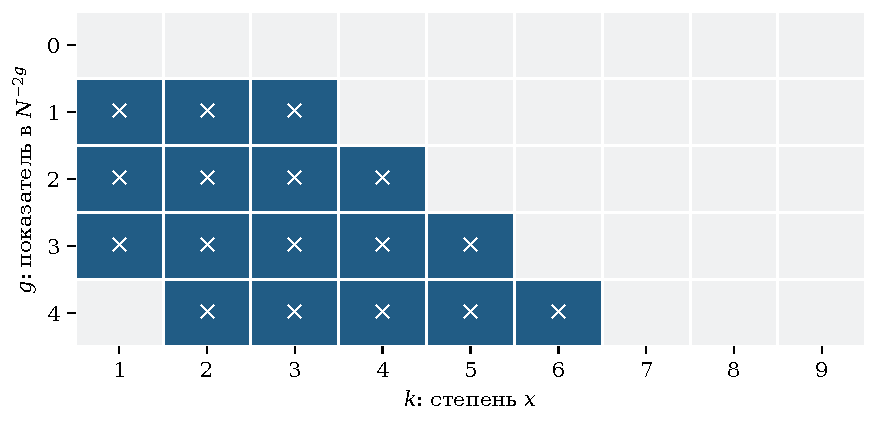
\includegraphics[width=.85\linewidth]{coefficient_grid.pdf}
\caption{Ненулевые препятствия для коэффициентов
$[N^{-2g}x^k]$ на девятихордовом сертификате. Крестом отмечены
17 установленных ненулевых значений. Светлые клетки не означают
доказанной продолжимости.}
\end{figure}

\section{\texorpdfstring{Коэффициенты примитивного $\sll_2$-веса}{Коэффициенты примитивного sl(2)-веса}}
\label{sec:sl2}

\subsection{Уточнённая задача}

Далее форма на $\sll_2$ --- форма Киллинга; переменная $c$ обозначает
её квадратичный Казимир. На неприводимом представлении старшего веса $a$
он действует числом $a(a+2)/8$. Рассматривается функция
\begin{equation}\label{eq:Fn}
 F_n(D)=[c^{\lfloor(n-1)/2\rfloor}]\,w_{\sll_2}(\pi(D)).
\end{equation}
Вопрос состоит в существовании линейного графового 4-инварианта
порядка $n$, совпадающего с $F_n$ на графах пересечений.
Ни мультипликативность, ни единственность продолжения не предполагаются.

Здесь принципиальна проекция $\pi$. Добавление изолированной хорды
умножает обычный вес на $c$, но даёт произведение положительных степеней,
которое убивается примитивной проекцией. Поэтому перенос обычного
9-вершинного препятствия умножением на $c$ не отвечает на
\eqref{eq:Fn}.

\begin{theorem}\label{thm:extension}
Для каждого $n\in\{11,12,13,14\}$ функция \eqref{eq:Fn}
не продолжается до графового 4-инварианта.
\end{theorem}
Доказательство для нечётных порядков использует оценку размерности
примитивного графового фактора и точный конечный сертификат.
Чётные порядки получаются корректным добавлением листа.
Ниже приведены все теоретические переходы, необходимые для вывода
из вычисленных матриц.

\subsection{Фурье-описание графовых 4T}

Маркированные графы на $n$ вершинах образуют векторное пространство
$\F_2^{\binom n2}$ с координатами $A_{ij}$.
Пусть $T_{ab}$ добавляет координаты $A_{bv}$ к $A_{av}$ при
$v\ne a,b$, сохраняя остальные. Через $E_{ab}$ обозначим
переключение ребра $ab$. Эти преобразования коммутируют.
Графовые 4T имеют вид
\[
 \Delta_{ab}f(A)=\Delta_{ab}f(T_{ab}A),\qquad
 \Delta_{ab}f(A)=f(A)-f(A+E_{ab}).
\]
Рассмотрим преобразование Фурье
\[
 \widehat f(B)=\sum_A(-1)^{\sum_{i<j}A_{ij}B_{ij}}f(A).
\]
Оператор $\Delta_{ab}$ становится умножением на $2B_{ab}$.
Транспонированный к $T_{ab}$ оператор равен $T_{ba}$ и сохраняет
$B_{ab}$. Поэтому графовые 4T эквивалентны условию
\begin{equation}\label{eq:fourier}
 \widehat f(B)=\widehat f(T_{ba}B)\quad\text{при }B_{ab}=1.
\end{equation}
Это элементарные преобразования соседних базисных векторов
из классификации трансвекций над $\F_2$ \cite{seven}.
Фурье коммутирует с перестановками вершин, поэтому размерность
$\mathcal H_n$ равна числу классов графов относительно этих
преобразований и изоморфизмов.

\subsection{Размерность примитивного фактора}

Преобразования \eqref{eq:fourier} сохраняют компоненты связности.
При удалении ребра $a v$ остаётся обход через $b$, поскольку
$ab$ и $bv$ являются рёбрами; новые рёбра не выходят за пределы
старой компоненты. Пусть $t_r$ --- число классов связных графов
порядка $r$. Тогда класс произвольного графа задаётся мультимножеством
классов компонент, откуда
\begin{equation}\label{eq:hilbert}
 \sum_{n\ge0}\dim\mathcal H_n\,z^n
 =\prod_{r\ge1}(1-z^r)^{-t_r}.
\end{equation}
С другой стороны, связная градуированная коммутативная
кокоммутативная алгебра Хопфа над $\Q$ является симметрической
алгеброй на примитивных элементах. Её ряд Гильберта имеет вид
правой части \eqref{eq:hilbert} с показателями
$\dim\Prim(\mathcal H)_r$. Единственность эйлерова разложения даёт
\begin{equation}\label{eq:dim-connected}
 \dim\Prim(\mathcal H)_r=t_r.
\end{equation}
Здесь не предполагается, что преобразование Фурье является
изоморфизмом алгебр Хопфа; используются только размерности.

По классификации Brown--Humphries, изложенной в \cite{seven},
каждый связный граф эквивалентен дереву, а семейства на рисунках
2--5 этой работы дают полный набор представителей.
Theorem 3.3 и Proposition 3.4 позволяют получить следующую верхнюю
оценку числа представителей:
\begin{center}
\begin{tabular}{lcc}
\toprule
Семейство и условия&$n=11$&$n=13$\\\midrule
$D_{m,k}$: $m+k=n$, $m\ge2,k\ge1$&9&11\\
Рис. 3: $2r+p=n$, $r\ge3,p\ge0$&3&4\\
Рис. 4: $2r+p=n$, $r\ge4,p\ge0$&2&3\\
Рис. 5: $2r+p=n$, $r\ge3,p\ge1$&3&4\\\midrule
Всего&17&22\\\bottomrule
\end{tabular}
\end{center}
Для верхней оценки не требуется попарная различность всех
перечисленных представителей. Из \eqref{eq:dim-connected} следует
\begin{equation}\label{eq:dim-upper}
 \dim\Prim(\mathcal H)_{11}\le17,\qquad
 \dim\Prim(\mathcal H)_{13}\le22.
\end{equation}

\subsection{Графовые функционалы, заполняющие эту размерность}

Используются три мультипликативных полинома произвольного графа $G$:
\begin{align}
 U_G(N)&=N^{\corank A_G},\label{eq:graphU}\\
 P_G(N)&=\sum_{s\in\F_2^{V(G)}}(-1)^{|s|}
 N^{\operatorname{nullity}(A_G+\operatorname{diag}s)},\label{eq:graphP}\\
 S_G(N)&=\sum_{p:V(G)\to\binom{[N]}2}
 (-1)^{\sum_{uv\in E(G)}|p(u)\cap p(v)|}.\label{eq:graphS}
\end{align}
Матрицы в \eqref{eq:graphU}--\eqref{eq:graphP} рассматриваются над $\F_2$.
Полиномиальность $S_G$ следует группировкой назначений по реально
использованным цветам.

Для $U$ графовые 4T следуют из конгруэнции матрицы смежности:
$\widetilde A=TAT^t$ и $TET^t=E$ для переключаемого ребра.
Оба ранга в разности сохраняются.
Для $P$ та же конгруэнция даёт
\[
 T(A+\operatorname{diag}s)T^t
 =\widetilde A+\operatorname{diag}s'+s_bE_{ab},\qquad
 s'_a=s_a+s_b,\quad s'_i=s_i\ (i\ne a).
\]
При $s_b=1$ члены разности по ребру меняются местами, а знак
$(-1)^{|s|}$ также меняется. Эти два минуса сокращаются.
Получаем \eqref{eq:graph4t}.

Для $S$ в разности по ребру $ab$ остаются только назначения с
$|p(a)\cap p(b)|=1$. На них отображение
$p(b)\mapsto p(a)\mathbin\triangle p(b)$ --- инволюция на
двухэлементных множествах. Она меняет знаки ровно так, как
тильда-преобразование рёбер от $a$ к соседям $b$.
Это доказывает графовые 4T для каждого целого $N$, а значит,
и как полиномиальное тождество.

Для $M=U,P,S$ положим $K_M=M\circ\pi_{\mathcal H}=\log_*M$.
Каждый коэффициент $K_M(G;N)$ является функционалом на примитивном
графовом факторе. Степени $K_U,K_P$ не превосходят $n$.
Для $K_S$ достаточно степени $n+1$.

Последнюю границу можно доказать непосредственно. Запишем
$h(p,q)=(-1)^{|p\cap q|}-1$. Связное кластерное разложение кумулянта даёт
\[
 K_S(G;N)=\sum_p\sum_{\substack{A\subseteq E(G)\\(V(G),A)\ \text{связен}}}
 \prod_{uv\in A}h(p(u),p(v)).
\]
В ненулевом слагаемом соседние пары имеют ровно один общий цвет.
Вдоль остова корневая пара использует два цвета, каждая следующая
вершина добавляет не более одного. Всего используется не более
$n+1$ цветов. Группировка по числу цветов выражает $K_S$ в базисе
$\binom Nk$, $k\le n+1$.

\subsection{Точные сертификаты в порядках 11 и 13}

Для порядка 11 выбраны 18 хордовых диаграмм $D_i$, для порядка 13 ---
23 диаграммы. Строка матрицы $M_n$ содержит все коэффициенты
$K_U(\Gamma D_i)$, $K_P(\Gamma D_i)$ и $K_S(\Gamma D_i)$.
Для первых двух используется мономиальный базис, для последнего ---
биномиальный. Получены точные ранги над $\Q$:
\begin{center}
\begin{tabular}{ccccc}
\toprule
$n$&Размер $M_n$&$\rk M_n$&$\rk(M_n\mid F_n)$&Число диаграмм\\\midrule
11&$18\times37$&17&18&18\\
13&$23\times43$&22&23&23\\\bottomrule
\end{tabular}
\end{center}
В сочетании с \eqref{eq:dim-upper} это доказывает полноту выбранных
графовых функционалов: они порождают всё двойственное пространство
$\Prim(\mathcal H)_n^*$, а не только некоторое частное семейство.

В файлах сертификатов приведены слова $D_i$, рациональные
$\alpha_i$ и все полиномы. Положим $L_n=\sum_i\alpha_iD_i$.
Проверено точное покоэффициентное обнуление
\[
 \sum_i\alpha_i K_U(\Gamma D_i;N)=
 \sum_i\alpha_i K_P(\Gamma D_i;N)=
 \sum_i\alpha_i K_S(\Gamma D_i;N)=0.
\]
По полноте функционалов получаем
\begin{equation}\label{eq:primitive-kernel}
 \pi_{\mathcal H}\Gamma(L_n)=0.
\end{equation}
Но нужные коэффициенты не обнуляются:
\begin{align}
 F_{11}(L_{11})&=-\frac{3853}{16342},\label{eq:obstruction11}\\
 F_{13}(L_{13})&=-\frac{584516618797266710299103168}
 {315656869633392158362337}.\label{eq:obstruction13}
\end{align}

Предположим, что существует графовое продолжение $f$ функции $F_n$.
Можно заменить его на $f\circ\pi_{\mathcal H}$: на графах пересечений
значения не изменятся. Действительно, $F_n$ уже убивает произведения
положительных степеней, а все термы проекции графа пересечений снова
являются графами пересечений. Поэтому из \eqref{eq:primitive-kernel}
следовало бы
\[
 F_n(L_n)=f(\pi_{\mathcal H}\Gamma(L_n))=f(0)=0,
\]
что противоречит \eqref{eq:obstruction11} или
\eqref{eq:obstruction13}. Непродолжимость при $n=11,13$ доказана.

Сертификат здесь --- рациональная линейная комбинация примитивных
диаграмм. Не требуется предъявлять две диаграммы с одинаковым графом
и разными $\sll_2$-весами. Равенство \eqref{eq:primitive-kernel} также
не заменяется более сильным, не доказанным равенством
$\Gamma(L_n)=0$ до применения проекции.

\subsection{Добавление листа и чётные порядки}

Пусть $D^+$ получается добавлением хорды, пересекающей ровно одну
старую хорду. В нормировке Киллинга обычный вес умножается на
$c-\tfrac12$. Для примитивного веса при $|D|>0$ получаем
\begin{equation}\label{eq:leaf}
 w_{\sll_2}(\pi(D^+))=-\frac12w_{\sll_2}(\pi(D)).
\end{equation}
Один вывод использует нильпотентные производящие функции моментов.
Выделим переменную $x$ корневой хорды и переменную $y$ нового листа;
$x^2=y^2=0$. Если исходная функция моментов равна $M_0+xM_1$,
то новая равна
\[
 M^+=(1+cy)M_0+x(1+(c-\tfrac12)y)M_1.
\]
Коэффициент $xy$ в $\log M^+$ равен
$-\tfrac12 M_1/M_0$, тогда как коэффициент $x$ в $\log M$ равен
$M_1/M_0$. Выделение остальных вершин даёт \eqref{eq:leaf}.

Существенно и графовое утверждение: добавление листа задаёт корректную
операцию $\ell$ на примитивном графовом 4T-факторе и
\[
 \pi_{\mathcal H}(G^+)=\ell(\pi_{\mathcal H}G).
\]
Оно следует из Theorems 2.1--2.3 работы Карева \cite{karev}.
В модели с красными рёбрами примитивный образ представляется суммой
связных остовных подграфов; каждый связный остов $G^+$ обязан содержать
новое ребро-лист. Корректность операции по модулю отношений обеспечивается
указанной теоремой, а не одним лишь численным равенством весов.

Поэтому добавление листа к каждому слагаемому $L_{11}$ и $L_{13}$
сохраняет нулевой примитивный графовый образ. В парах порядков
$11,12$ и $13,14$ выделяется одна и та же степень $c$.
Из \eqref{eq:leaf} получаем ненулевые препятствия
\[
 F_{12}(L_{11}^+)=\frac{3853}{32684},\qquad
 F_{14}(L_{13}^+)=\frac{292258309398633355149551584}
 {315656869633392158362337}.
\]
Теорема~\ref{thm:extension} доказана.

\subsection{Что именно проверял компьютер}

Использована целочисленная нормировка
\[
 H_D(t)=8^n w_{\sll_2}(\pi(D))(t/8).
\]
Если $h_k=[t^k]H_D$, то $[c^k]w_{\sll_2}(\pi D)=h_k/8^{n-k}$.
Все полные полиномы диаграмм сертификатов пересчитаны рекурсией
Чмутова--Варченко. Для порядка 13 каждый из трёх графовых полиномов
дополнительно вычислен непосредственно на 13 вершинах, без переноса
готового значения с меньшего порядка.

Для $K_S$ использованы значения $N=0,\ldots,16$.
Первые 15 точек однозначно определяют многочлен степени не выше 14,
ещё две служат контролем. Моменты считаются как коэффициенты
\[
 S_G(N)=\Bigl[\prod_v x_v^2\Bigr]
 \left(\sum_{U\subseteq V}(-1)^{|E(G[U])|}\prod_{v\in U}x_v\right)^N
\]
в кольце $x_v^3=0$, затем применяется \eqref{eq:anchor}.
Это требует $O(n5^n)$ арифметических действий и $O(3^n)$ ячеек.
В промежуточных таблицах при $n=13,N\le16$ достаточно знакового
128-битного целого, поскольку их абсолютные значения не превосходят
$\binom{16}2^{13}<2^{127}$. Кумулянты хранятся в целых произвольной
точности, ранги вычисляются рациональным исключением.

Граница степени следует из PBW-представления~\cite{cdm} примитивной диаграммы
связными открытыми диаграммами Якоби. Если $u$ --- число ног, а $l$
--- число независимых циклов, то $n=u+l-1$. Связные деревья с одной
меткой, кроме распорки, исчезают по AS/IHX; при $l=1$ и нечётном $n$
число ног нечётно, и инвариантный полином $\sll_2$ равен нулю.
Поэтому максимальное ненулевое чётное $u$ равно $n-1$, а степень
по квадратичному Казимиру не больше $(n-1)/2$. Для $n=13$ это 6.

Независимая проверка всех 23 полных $H_D$ выполнена прямыми матрицами
представлений $\sll_2$ старших весов $a=1,\ldots,8$.
Сворачивается тензор
\[
 8\Omega=2E\otimes F+2F\otimes E+H\otimes H.
\]
Матричные моменты всех поддиаграмм дают примитивные значения в точках
$t=a(a+2)$. Теоретическая граница примитивной степени в порядке 13
равна 6. Точки $a=1,\ldots,6$ вместе с нулём восстанавливают полный
полином; $a=7,8$ --- дополнительные проверки. Все коэффициенты совпали
с хордовой рекурсией. Таким образом, вычислительная часть не сводится
к повторной подстановке в тот же самый рекурсивный результат.

Сертификаты и программы составляют конечную проверяемую часть
доказательства. Теоретические части --- \eqref{eq:fourier},
\eqref{eq:dim-connected}, классификационная оценка,
графовые 4T для $U,P,S$, полнота функционалов и перенос листом ---
не заменяются сообщением программы об успешном тесте.

Доказан отрицательный ответ для каждого порядка от 11 до 14.
Утверждение о всех $n\ge15$ или о существовании некоторого
асимптотического порога этим доказательством не устанавливается.

\section{Воспроизведение результатов}

Исходники, точные многочлены и сертификаты размещены в репозитории
\href{https://github.com/TheMrX1/gl-weight-systems}{TheMrX1/gl-weight-systems}.
В нём отделены вычислительное ядро, конечные сертификаты и текст.
Для сборки нужны CMake 3.24+, компилятор C++20 с поддержкой
128-битных целых (Clang или GCC), заголовки Boost.JSON и
Boost.Multiprecision, Python 3.10+. Рисунки используют Matplotlib.
Черновик PDF собирается Tectonic; исходник использует русский язык,
шрифт Times New Roman и обычные пакеты AMS.

Из папки клонированного репозитория:
\begin{Verbatim}[fontsize=\small]
cmake -S . -B build -DCMAKE_BUILD_TYPE=Release \
  -DBOOST_ROOT=/path/to/boost
cmake --build build --parallel 3
python3 scripts/verify_results.py --matrix
ctest --test-dir build --output-on-failure
\end{Verbatim}
Путь к Boost задаётся только если заголовки не обнаружены автоматически.

Для введённой диаграммы:
\begin{Verbatim}[fontsize=\small]
build/evaluate_word --specialization gl "0 1 0 1"
build/gl_polynomial --primitive-polynomial "0 1 0 1"
printf '%s\n' "0 1 0 1" | build/sl2_word_batch
\end{Verbatim}
Первая команда вычисляет три значения универсального gl-веса,
вторая --- полный обычный и примитивный gl-полиномы,
третья --- примитивный $\sll_2$-полином в нормировке $H_D$.
Это разные вычисления, их результаты не следует сравнивать без
согласования специализации и нормировки.

Основные группы файлов:
\begin{center}\small
\begin{tabularx}{\linewidth}{@{}lX@{}}
\toprule
Путь&Содержание\\\midrule
\file{cpp/}&Ядро и самостоятельные C++-вычислители\\
\file{results/mutants11/}&Четыре слова, обычные и примитивные gl-полиномы\\
\file{results/mutants14/}&Сертификат четырёх различных скалярных весов\\
\file{results/K11/}&Полный $K_{11}$ и бесследовые вспомогательные полиномы\\
\file{results/hooks/}&Коэффициентные сертификаты формул для крюков\\
\file{results/graphs9/}&Хроматические и прямоугольные специализации\\
\file{certificates/order9/}&Развёрнутый авторский графовый сертификат\\
\file{certificates/order11/}&18 диаграмм и рациональные коэффициенты\\
\file{certificates/order12/}&Перенос сертификата добавлением листа\\
\file{certificates/order13/}&23 диаграммы, полиномы и матричные проверки\\
\file{scripts/}&Проверки, реконструкция и построение рисунков\\
\file{report/}&Настоящий текст, PDF и исходные изображения\\\bottomrule
\end{tabularx}
\end{center}

В быстрых проверках заново вычисляются все sl(2)-полиномы
сертификатов порядков 11--14 и выполняются точные проверки
сохранённых универсальных gl-полиномов. Получение последних
с нуля является отдельным, более тяжёлым запуском.
Размеры диаграмм и параметры подстановок во всех сертификатах
зафиксированы явно; проверка сохранённого результата и его новый
расчёт в инструкциях различаются.

\begin{thebibliography}{9}
\bibitem{yang}
Z. Yang. \emph{New approaches to $\mathfrak{gl}_N$ weight system}.
\href{https://arxiv.org/abs/2202.12225}{arXiv:2202.12225}.

\bibitem{chmutovlando}
S. Chmutov, S. Lando. \emph{Mutant knots and intersection graphs}.
Algebraic \& Geometric Topology \textbf{7} (2007), 1579--1598.
\href{https://arxiv.org/abs/0704.1313}{arXiv:0704.1313}.

\bibitem{kkl}
M. Kazarian, N. Kodaneva, S. Lando.
\emph{The universal $\mathfrak{gl}$-weight system and the chromatic polynomial}.
\href{https://arxiv.org/abs/2406.10562}{arXiv:2406.10562}.

\bibitem{fkpu}
D. Fomichev, M. Karev, F. Pavutnitskiy, S. Usanov.
\emph{$\mathfrak{sl}(2)$-weight system does not extend to a graph 4-invariant}.
\href{https://arxiv.org/abs/2607.24217}{arXiv:2607.24217}.
Авторский сертификат используется с указанием происхождения данных.

\bibitem{seven}
A. I. Seven. \emph{Orbits of groups generated by transvections over $\mathbb F_2$}.
\href{https://arxiv.org/abs/math/0303098}{arXiv:math/0303098v2}.
Definition 3.1, Theorem 3.3, Proposition 3.4 и рисунки 2--5.

\bibitem{karev}
M. Karev. \emph{On the primitive subspace of the Lando framed graph bialgebra}.
Communications in Mathematics \textbf{31} (2023), no. 3, 125--136.
\href{https://arxiv.org/abs/2307.00468}{arXiv:2307.00468}.
Theorems 2.1--2.3.
\bibitem{cdm}
S. Chmutov, S. Duzhin, J. Mostovoy.
\emph{Introduction to Vassiliev Knot Invariants}.
Cambridge University Press, 2012. Главы об алгебре диаграмм Якоби,
PBW-симметризации и Lie-весовых системах.
\end{thebibliography}
\end{document}
